\section{ヒストグラム}

\begin{frame}[t,fragile]{ヒストグラムの作り方}
  \begin{itemize}
    %\setlength{\itemsep}{1em}
  \item 連続変数(実数)のデータの場合 ([]内はサンプルプログラムでの変数名)
    \begin{itemize}
    \item $N$: サンプル数 [{\tt samples}]
    \item $x_{\rm min}$: データの最小値(カットオフ) [{\tt xmin}]
    \item $x_{\rm max}$: データの最大値(カットオフ) [{\tt xmax}]
    \item $n$: ビンの個数 [{\tt bins}]
    \item $\Delta$: ビンの幅 ($\Delta=(x_{\rm max}-x_{\rm min}) / n$) [{\tt dx}]
    \end{itemize}
  \item サイズ$n$の配列を準備
    \begin{itemize}
    \item データ毎にどのビンに入るか計算: $j = (x - x_{\rm min}) / \Delta$
    \item (必要に応じて) $0 \le j < n$であることを確認 (範囲外のデータは無視する)
    \item 配列の$j$番目の値を1増やす
    \end{itemize}
    \item サンプルプログラム: \href{https://github.com/todo-group/computer-experiments/blob/master/exercise/monte_carlo/histogram.c}{histogram.c}
  \end{itemize}
  \vspace*{-5cm} \hfill \resizebox{0.28\textwidth}{!}{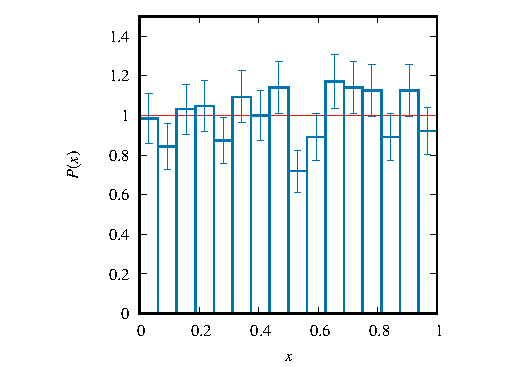
\includegraphics{image/histogram.pdf}}
\end{frame}

\begin{frame}[t,fragile]{ビンの個数の設定}
  \begin{itemize}
  \item 最適の幅というものはない
  \item 個数を増やすと表現の自由度は増えるが、各ビンのエラーバーが大きくなる
    \begin{itemize}
    \item データが統計的に独立である場合、それぞれのビンのカウント数$m$はポワソン分布に従う
    \item 統計誤差 $\sim \sqrt{m}$
    \end{itemize}
  \item いくつかの方法・公式が提案されているが、分布の形によっては不適切な場合も
    \begin{itemize}
    \item スタージェスの公式 $n = \log_2 N + 1$
    \item スコットの公式 $\Delta = 3.5 \sigma / N^{1/3}$
    \end{itemize}
  \item 実際には、ビンの個数を何通りか試してみるのが良い
  \item データを取り直すことが出来ない and/or コストがかかる場合も多いので、生データはいったんファイルに保存しておく
  \end{itemize}
\end{frame}
